\documentclass{fefu}
\usepackage{float}
\usepackage{algorithm}% http://ctan.org/pkg/algorithms
\usepackage{algpseudocode}% http://ctan.org/pkg/algorithmicx
\author{Терехов Д.Е.}
\setschool{ШКОЛА ЕСТЕСТВЕННЫХ НАУК ДВФУ}
\setdepartment{кафедра информатики, математического и компьютерного моделирования}{Чеботарев}
\setgroup{Б8403а}
\begin{document}
\makereporttitle
\tableofcontents
\pagebreak
\section*{Аннотация}
В компьютерной графике объекты состоят из полигонов, чаще всего треугольников.
На видеокарту загружается текстурный атлас -- совокупность текстур меньшего размера.
Для уменьшения количества текстурных атласов и вызовов на отрисовку необходимо как можно плотнее упаковать
текстуры в атласы. Для этого предварительно текстуры необходимо триангулировать текстуры -- таким образом
 она будет занимать меньшее пространство, а также фрагментному шейдеру необходимо будет отрисовать меньше пикселей.
\section{Введение}
\subsection{Глоссарий}
\begin{itemize}
    \item online-алгоритм -- блаблабла
    \item Окрестность Мура клетки — в двумерном случае — совокупность восьми клеток на квадратном паркете,
    имеющих общую вершину с данной клеткой.
\end{itemize}
\subsection{Описание предметной области}
\subsubsection{Студия "Game Forest"}
Работа выполняется по заказу студии "Game Forest". TODO
\subsubsection{Citrus Game Engine}
Citrus -- игровой движок с открытым исходным кодом, распространяемый по лицензии GPL-3.0.
репозиторий размещен на платформе Github \cite{CitrusRepo}. Citrus Game Engine
состоит из следующих компонент:
\begin{itemize}
    \item Lime -- ядро игрового движка
    \item Lemon -- линкер сторонних библиотек
    \item Yuzu -- библиотека для сериализации
    \item Orange -- сборщик приложений
    \item Tangerine -- редактор сцен
    \item Kumquat -- генератор кода
\end{itemize}
\subsubsection{Полигонализация текстур и PolygonMesh виджет}
В игровом движке Citrus существуют посредственные методы для работы с полигональным мешем --
DistortionMesh виджет. Проблема такого подхода заключается в табличном задании меша (пересечение столбца и строки --
вершина меша) и в том, что каждая вершина сама по себе является узлом (Node) в иерархии объектов, что очень сильно сказывается на
производительности DistortionMesh. Были предложены следующие подходы к решению проблемы:
\begin{itemize}
    \item Попытаться оптимизировать текущую реализацию DistortionMesh
    \item Избавиться от представления вершин в виде узлов в иерархии объектов
    \item Создать новый виджет PolygonMesh, лишенный всех проблем DistortionMesh
\end{itemize}
Бесспорно, было принято решение разработать новый виджет PolygonMesh. Для того чтобы вершины могли
иметь не предопределённые позиции, необходимо поддерживать специальную структуру представляющую собой
полигонализацию множества точек, что является моей частью работы по созданию PolygonMesh виджета. Были выдвинуты
следующие требования к методам полигонализации множества точек:
\begin{itemize}
    \item Полигоном является треугольник (поэтому далее будет применятся термин триангуляция), т.к.
треугольники чаще всего используются в компьютерной графике
    \item Алгоритм триангуляции должен быть online
    \item Алгоритм триангуляции должен быть достаточно быстрым, чтобы использовать его в редакторе сцен
    Tangerine для нового виджета PolygonMesh
\end{itemize}
Разработанные методы триангуляции используются в работе Гоменюка А.А. "Редактор текстурного меша и его скелетная анимация
при помощи шейдеров в игровом движке Citrus".
\subsubsection{Упаковка текстур в атласы}
Для того чтобы уменьшить количество вызовов на отрисовку текстуры пакуются в текстурные атласы. Чем меньше атласов на
то же самое количество текстур, тем:
\begin{itemize}
    \item Игра занимает меньший размер
    \item Происходит меньше вызовов на отрисовку
    \item Расходуется меньше видеопамяти
\end{itemize}
Для упаковки текстур в игровом движке Citrus используется жадный алгоритм. Было предложено несколько подходов для
оптимизации упаковки текстур в атласы:
\begin{itemize}
    \item Другой жадный алгоритм
    \item Жадный алгоритм и построение невыпуклой оболочки текстуры с дальнейшим превращением в полигональный меш
    \item Генетический алгоритм и построение невыпуклой оболочки текстуры с дальнейшим превращением в полигональный меш
\end{itemize}
Построение невыпуклой оболочки с дальнейшей триангуляцией способно уменьшить площадь, занимаемую текстурой, что
может способствовать лучшей упаковке текстуры в атлас. Было предложено написать другой жадный алгоритм для упаковки
прямоугольных текстур, а также провести эксперимент: для каждой текстуры построить невыпуклую оболочку, триангулировать
её, написать генетический алгоритм для упаковки полигональных текстур. Если эксперимент покажет, что данный подход во
много раз превосходит другие, то в дальнейшем планируется провести ряд других экспериментов, положительный результат
которых, позволит внедрить данную работу в master игрового движка Citrus.
\subsection{Неформальная постановка задачи}
В рамках работы требуется:
\begin{itemize}
    \item Реализовать методы для работы с триангуляцией множества точек (вставка, удаление, перемещение вершин)
    \item Реализовать алгоритм\textbackslash ы для генерации невыпуклой оболочки текстуры
\end{itemize}
\subsection{Обзор существующих решений}
\subsubsection{Триангуляция}
Некоторые математические программные пакеты (plotly, scipy, matlab) предоставляют возможности по триангуляции
множества точек. Однако они не подходят для поставленной задачи по ряду причин:
\begin{itemize}
    \item Написаны на "медленных" языках программирования
    \item Вынуждают подтягивать за собой огромное количество не нужны пакетов
    \item Предоставляют только offline алгоритмы
\end{itemize}
Также существует библиотека Triangle \cite{TriangleSite}, написанная Jonathan Richard Shewchuk на языке С, и
обертка на C\# Triangle.NET. К сожалению, обертка добавляет слишком много недопустимых зависимостей в проект и не
предоставляет online алгоритм. Создание своей обертки на Triangle вызывает большие трудности по поддержке
кроссплатформенности и переписыванию части большой части кода. К тому же, некоторых нужных методов триангуляции в
данной библиотеке не оказалось.
\subsubsection{Генерация невыпуклой оболочки}
Spine предоставляет возможность сгенерировать меш для текстуры (с предварительной генерацией, возможно, невыпуклой оболочки).
Это единственное найденное конкурирующее решение.
\section{Математические методы}
\subsection{Трассировка контура}
Одним из способов генерации невыпуклой оболочки объекта $I$, представленного на текстуре, является выявление
его контура $B$ (границы) и дальнейшее аппроксимация контура полигоном. Введем несколько понятий. Будем считать
пиксель белым, если он не принадлежит объекту, контур которого мы хотим выделить, черным в противном случае.
В каждом из нижеприведенных алгоритмов находится начальный пиксель. Будем считать начальным пикселем самый левый
нижний черный пиксель.
\subsubsection{Square tracing}
Идея данного алгоритма проста: если текущий пиксель черный, то нужно добавить его к множеству точек границы $B$,
повернуть налево и сделать шаг вперед, иначе повернуть направо и сделать шаг вперед. Следующий псевдокод
описывает данный алгоритм:
\begin{algorithm}
    \caption{Square tracing}
    \begin{algorithmic}[1]
        \Procedure{SquareStrace}{$I$} \Comment{I is set of pixels}
            \State $start \gets GetStartPixel(I)$
            \State $B \gets \{start\}$
            \State $direction \gets \left(0, -1\right)$
            \State $next \gets start + direction$
            \While{$next \not= start$}
                \If{next is BLACK}
                    \State $B \gets B \cup \{p\}$
                    \State $direction \gets TurnLeft(direction)$
                \Else
                    \State $direction \gets TurnRight(direction)$
                \EndIf
                \State $next \gets next + direction$
            \EndWhile
            \State \textbf{return} $B$
        \EndProcedure
    \end{algorithmic}
\end{algorithm}
\subsubsection{Трассировка окрестности Мура}
Общая идея такова: каждый раз, когда вы наступаете на черный пиксель $p$, возвращайтесь назад, т.е. возвращайтесь к белому
пикселю $c$, на котором стояли ранее, затем по часовой стрелке посещается каждый пиксель в окрестности Мура (рис. 1)
пикселя $p$, пока не найден черный пиксель. Алгоритм заканчивается, когда начальный пиксель посещается во второй раз.
Посещенные черные пиксели образуют контур.
\begin{figure}[H]
    \centering
    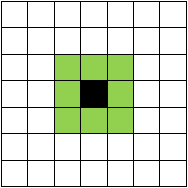
\includegraphics[scale=0.7]{images/MooreNeighbourhood.png}
    \caption{Окрестность Мура}
\end{figure}
\begin{algorithm}
    \caption{Moor neighborhood tracing}
    \begin{algorithmic}[1]
        \Procedure{MoorNeighborhoodTrace}{$I$} \Comment{I is set of pixels}
            \State $start \gets GetStartPixel(I)$
            \State $B \gets \{start\}$
            \State $p \gets start$
            \State $c \gets NextMoorNeighbor\left(p + \left(0, 1\right)\right)$
            \While{$c \not= start$}
                \If{c is BLACK}
                    \State $B \gets B \cup \{c\}$
                    \State $p \gets c$
                    \State $c \gets PrevMoorNeighbor(c)$
                \Else
                    \State $c \gets NextMoorNeighbor(c)$
                \EndIf
            \EndWhile
            \State \textbf{return} $B$
        \EndProcedure
    \end{algorithmic}
\end{algorithm}
\subsection{Генерация невыпуклой оболочки}
\subsubsection{Visvalingam line simplification algorithm}
\subsubsection{4 point ?}
\subsection{Триангуляция}
Сравнение разных видов триангуляции, выбор Делоне, описание структур данных, описание юыважываж
\subsection{Bin packing problem}
Жадник + генетика
\newpage
\bibliographystyle{ugost2008ls}
\bibliography{references}
\end{document}
